\documentclass[a4paper]{article} %

\date{} %

% Please, do not change any of the above lines

\usepackage{amssymb} % add other LaTeX packages you need here.

% extra packages
\usepackage{tikz}
\usepackage{amssymb}
\usepackage{verbatim} % for comment


\newtheorem{theorem}{Theorem}
\newtheorem{problem}[theorem]{Problem}

%%%%


\begin{document}
\setcounter{page}{1} % Please, do not delete this line

% Your title
\title{Quasi-equational bases for directed paths}

% Authors
\author{Marcel Jackson \\ %
       La Trobe University, Melbourne, Australia\\ \\ % Affiliation 1
       Tomasz Kowalski \\ % If any other author with different Affilation
       Jagiellonian University, Krak\'ow,
   Poland\\ \\ % Affiliation 2 (if needed)
        Michał Stronkowski \\
        Warsaw University of Technology,
   Warsaw, Poland \\
       % Add authors and affiliation as needed
       \texttt{michal.stronkowski@pw.edu.pl} % Only one corresponding e-mail, please
       }%

\maketitle

% The abstract

For a finite relational structure $P$, let $Q(P)$ and  be the class of 
all relational structures isomorphic to an induced  
 substructure of a power of
$P$.  The class $Q(P)$ is axiomatizable by \emph{quasi-identities}, i.e., sentences of the form  
\[
(\forall \bar x)\; [\varphi_1(\bar x)\land\cdots\land\varphi_n(\bar
x)\Rightarrow \varphi(\bar x)],  
\]
where $\varphi_i$, $\varphi$ are atomic formulas. In digraphs these are of the
form $x\to y$ (there is an edge from $x$ to $y$) and $x=y$.   
%We call such sentences \emph{quasi-identities}, for historical reasons.
Then $P$ is \emph{finitely q-based}  if
$Q(P)$ is axiomatizable by a finite number of 
quasi-identities. We study the \mbox{following question.}

\begin{problem}
Which finite relational structures are finitely q-based?
\end{problem}

Related questions for finite algebras have stimulated research in universal algebra for decades. Perhaps the most prominent result in this direction is McKenzie's solution to Tarski's problem.%: it is undecidable whether a given finite algebra is finitely based, i.e., whether the variety it generates is finitely axiomatizable 
\cite{McK96}. Deep results were also obtained for quasivarieties, see e.g. \cite{Dzi09,Pig88}.
However the results for
relational structures are rare. As an example we recall Pultr's and Ne\v set\v
ril's theorem stating that the only finitely q-based finite simple graphs are disjoint
unions of complete bipartite graphs \cite{Cai95}.  

In the hope of discovering a general pattern, we decided to look closer at a class
of digraphs that, on one side, behave essentially different than simple graphs
and, on the other, are not too complicated. We focus on \emph{directed paths}, 
that is, digraphs obtained from a path in a simple graph by
choosing a direction for each of its edges. One may visualize directed paths
by Hasse-like diagrams where arrows are edges whose direction
is always upwards.%, see below for examples.  

\begin{center}
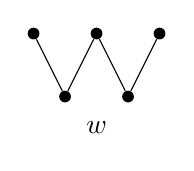
\begin{tikzpicture}[scale=0.8]\label{w}
\tikzset{v/.style={circle,fill,inner sep=1.5pt}}

\path (0,1) node[v] (b0) {};
\path (0.5,0) node[v] (a0) {};
\path (1,1) node[v] (b1) {};
\path (1.5,0) node[v] (a1) {};
\path (2,1) node[v] (b2) {};

\draw (a0) -- (b0);
\draw (a0) -- (b1);
\draw (a1) -- (b1);
\draw (a1) -- (b2);
\node at (1,-0.5) {$w$};
\end{tikzpicture}
\quad\quad
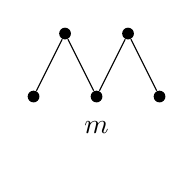
\begin{tikzpicture}[scale=0.8]
\tikzset{v/.style={circle,fill,inner sep=1.5pt}}

\path (0,0) node[v] (b0) {};
\path (0.5,1) node[v] (a0) {};
\path (1,0) node[v] (b1) {};
\path (1.5,1) node[v] (a1) {};
\path (2,0) node[v] (b2) {};

\draw (a0) -- (b0);
\draw (a0) -- (b1);
\draw (a1) -- (b1);
\draw (a1) -- (b2);
\node at (1,-0.5) {$m$};

\end{tikzpicture}
\quad\quad
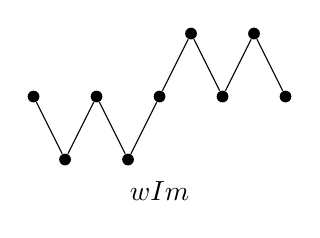
\begin{tikzpicture}[scale=0.8]
\tikzset{v/.style={circle,fill,inner sep=1.5pt}}

\path (0,1) node[v] (b0) {};
\path (0.5,0) node[v] (a0) {};
\path (1,1) node[v] (b1) {};
\path (1.5,0) node[v] (a1) {};
\path (2,1) node[v] (b2) {};
\path (2.5,2) node[v] (c0) {};
\path (3,1) node[v] (b3) {};
\path (3.5,2) node[v] (c1) {};
\path (4,1) node[v] (b4) {};

\draw (a0) -- (b0);
\draw (a0) -- (b1);
\draw (a1) -- (b1);
\draw (a1) -- (b2);
\draw (b2) -- (c0);
\draw (b3) -- (c0);
\draw (b3) -- (c1);
\draw (b4) -- (c1);

\node at (2,-0.5) {$wIm$};
\end{tikzpicture}

\mbox{}

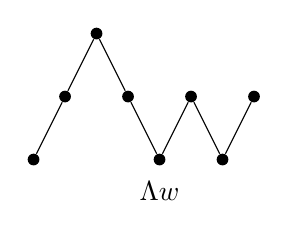
\begin{tikzpicture}[scale=0.8,v/.style={circle,fill,inner sep=1.5pt}]
\node[v] (a0) at (0,0) {};
\node[v] (b0) at (0.5,1) {};
\node[v] (c0) at (1,2) {};
\node[v] (b1) at (1.5,1) {};
\node[v] (a1) at (2,0) {};
\node[v] (b2) at (2.5,1) {};
\node[v] (a2) at (3,0) {};
\node[v] (b3) at (3.5,1) {};

\draw (a0)--(b0)--(c0)--(b1)--(a1)--(b2)--(a2)--(b3);

\node at (2,-0.5) {$\Lambda w$};
\end{tikzpicture}
\quad\quad
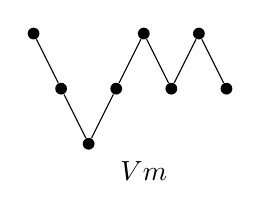
\begin{tikzpicture}[scale=.7,v/.style={circle,fill,inner sep=1.5pt}]
\node[v] (a0) at (0,2) {};
\node[v] (b0) at (0.5,1) {};
\node[v] (c0) at (1,0) {};
\node[v] (b1) at (1.5,1) {};
\node[v] (a1) at (2,2) {};
\node[v] (b2) at (2.5,1) {};
\node[v] (a2) at (3,2) {};
\node[v] (b3) at (3.5,1) {};

\draw (a0)--(b0)--(c0)--(b1)--(a1)--(b2)--(a2)--(b3);

\node at (2,-0.5) {$Vm$};
\end{tikzpicture}
\end{center}




Our most general result%, to be presented during the talk, 
has a rather technical formulation. But, during the talk, we will be mainly focused on proof technique that allows answering question in Problem 1, at least in some cases. Namely the lack of a finite q-base may be witnessed by the existence of an infinite family of so called critical digraphs.


Then is not difficult to show that 
if an directed path $P$
% such that $Q_I(P)$ 
contains one of $wIm$, $\Lambda w$ or $Vm$ (see the picture above), then $P$ is not
finitely $q$-based. 
%Similarly, if  $Q(P)$ contains one of $wIm$, $\Lambda w$ or $Vm$, then $P$ is not finitely efq-based.  
Let us consider directed paths that contain $w$ or $m$
but $\{wIm, \Lambda w, Vm\}\cap Q(P) = \emptyset$. We call them
valleys and hills. 
Critical digraphs relative to valleys and hills may be very complex. 
As a not complicated examples, consider \mbox{the following valleys}   
\begin{center}
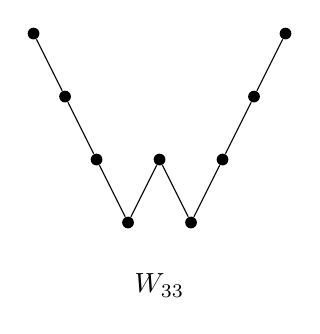
\begin{tikzpicture}[scale=0.8]
\tikzset{v/.style={circle,fill,inner sep=1.5pt}}

\node[v] (0) at (-1,3) {};
\node[v] (1) at (-.5,2)  {};
\node[v] (2) at (0,1)  {};
\node[v] (3) at (0.5,0)  {};
\node[v] (4) at (1,1)  {};
\node[v] (5) at (1.5,0)  {};
\node[v] (6) at (2,1)   {};
\node[v] (7) at (2.5,2)   {};
\node[v] (8) at (3,3)   {};
\draw (0) -- (1)--(2)--(3)--(4)--(5)--(6)--(7)--(8);
\node at (1,-1) {$W_{33}$};
\end{tikzpicture}
\quad\quad\quad
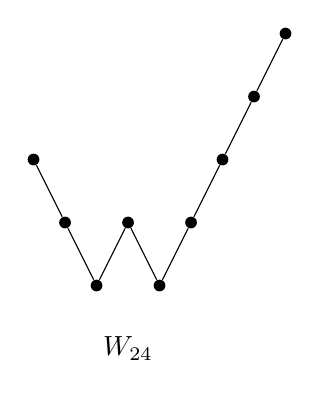
\begin{tikzpicture}[scale=0.8]
\tikzset{v/.style={circle,fill,inner sep=1.5pt}}

%\node[v] (0) at (-1,3) {};
\node[v] (1) at (-.5,2)  {};
\node[v] (2) at (0,1)  {};
\node[v] (3) at (0.5,0)  {};
\node[v] (4) at (1,1)  {};
\node[v] (5) at (1.5,0)  {};
\node[v] (6) at (2,1)   {};
\node[v] (7) at (2.5,2)   {};
\node[v] (8) at (3,3)   {};
\node[v] (9) at (3.5,4)   {};
\draw (1)--(2)--(3)--(4)--(5)--(6)--(7)--(8)--(9);
\node at (1,-1) {$W_{24}$};
\end{tikzpicture}
\end{center}
Then $W_{33}$ is finitely %(ef)
q-based while $W_{24}$ is not. The latter fact is witnessed by the depicted infinite family of  critical digraphs relative to $W_{24}$:

%\vspace{1em}

\begin{center}
\begin{tikzpicture}[scale=0.8]
\tikzset{v/.style={circle,fill,inner sep=1.5pt},dot/.style={circle,fill,inner sep=0.6pt}}

\node[v] (0) at (-1,3) {};
\node[v] (1) at (-.5,2)  {};
\node[v] (2) at (0,1)  {};
\node[v] (3) at (0.5,0)  {};
\node[v] (4) at (1,1)  {};
\node[v] (5) at (1.5,0)  {};
\node[dot] (d1) at  (2.5,0.5) {};
\node[dot] (d2) at (3,0.5) {};
\node[dot] (d3) at  (3.5,0.5) {};

\node[v] (4') at (4.5,1)  {};
\node[v] (5') at (5,0)  {};
\node[v] (6) at (5.5,1)   {};
\node[v] (7) at (6,2)   {};
\node[v] (8) at (6.5,3)   {};
\draw (0) -- (1)--(2)--(3)--(4)--(5);
\draw (4')--(5')--(6)--(7)--(8);
%\node at (1,-1) {Critical digraphs relative to $W_{33}$};
\end{tikzpicture}
\end{center}




\begin{thebibliography}{99}
\bibitem{Cai95}
X.~Caicedo.
\newblock Finitely axiomatizable quasivarieties of graphs.
\newblock {\em Algebra Univers.}, 34(2):314--321, 1995.

\bibitem{Dzi09}
Wies{\l}aw Dziobiak, Mikl{\'o}s Mar{\'o}ti, Ralph McKenzie, and Anvar
  Nurakunov.
\newblock The weak extension property and finite axiomatizability for
  quasivarieties.
\newblock {\em Fundam. Math.}, 202(3):199--223, 2009.

\bibitem{McK96}
Ralph McKenzie.
\newblock Tarski's finite basis problem is undecidable.
\newblock {\em Int. J. Algebra Comput.}, 6(1):49--104, 1996.

\bibitem{Pig88}
Don Pigozzi.
\newblock Finite basis theorems for relatively congruence-distributive
  quasivarieties.
\newblock {\em Trans. Am. Math. Soc.}, 310(2):499--533, 1988.


\end{thebibliography}

\end{document}
